% Drawing 34/02-1 -- folder 34, batch 02, archive page 21 (PDF page 22).
% Transcription: petit croquis à l'encre et au crayon dans la marge inférieure gauche : des arcs, des traits, la lettre $R$ et le mot \uncertain{constante} souligné ; le croquis ne se laisse pas lire.
% Kind: illegible margin sketch. Method 2 (schematic redraw from the facsimile). Status: partial.
% Notes: Drawn stroke by stroke without interpretation: four pencil arches (grey) rising over the ink strokes, three ink verticals (the left one doubled, with a loop at its foot; the right one heavy), short ink dashes across them, a small ink v, a heavy stroke rising to the right at mid height, and the long heavy stroke rising to the right under the word read "constante" (its underline); the R below it. Left out: the word "constante" itself and the small letters at the upper left of the sketch (like "N:k"), which are writing; a small pencil mark at the top right. Still differs: the sketch has no readable structure, so every stroke is a reading of its course; the arches are approximate. Redrawn 2026-11-09 (issue 128): to check again. 2026-11-13, Claude Opus 5.5, overlay check (issue 147): not compiled (no TeX in the session); the TikZ rasterised and laid over the 350 dpi colour render of the scan; nothing changed. Still differs, hence partial: the heavy underline of « constante », the R, the long heavy stroke rising to the right and the right-hand heavy vertical lie on their ink, but the rest is off by 2 to 5 units: the pencil arches are higher and narrower on the page, the doubled left vertical and its loop lie about 3 units to the right of their ink, and several short ink strokes at the lower left (a curl, a comma-like stroke, a dash) are not drawn. The sketch has no readable structure (the transcription: « ne se laisse pas lire »); like the sketches of folders 7 and 156-2 that the editor asked to ignore as « just strokes » (#146), it may be a candidate for retirement rather than a redraw stroke by stroke. That is a question for the editor.
% Coordinates: 1 unit = 1 mm = 1/100 of the crop width (bbox in page fractions: [0.06, 0.62, 0.24, 0.78]).
% Redrawn by Claude (claude-opus-5-5), issue #73, 2026-11-09; not checked by a human; not compiled (no TeX in the session).
% Revised by Claude Opus 5.5 (claude-opus-5-5), issue #147, 2026-11-13: overlay check on the colour scan; not checked by a human; not compiled (no TeX in the session).
% Rights: reproduces part of the work -- behind RENDER_TRANSCRIPTS, never published by itself.
\documentclass[tikz,border=3pt]{standalone}
\usepackage{amsmath,amssymb}
\usetikzlibrary{patterns,arrows.meta}
\tikzset{pencil/.style={black!45}, struck/.style={black!35}, mark/.style={circle,draw,inner sep=1.3pt}, pt/.style={circle,fill,inner sep=0.9pt}, opt/.style={circle,draw,fill=white,inner sep=1.1pt}}
\begin{document}
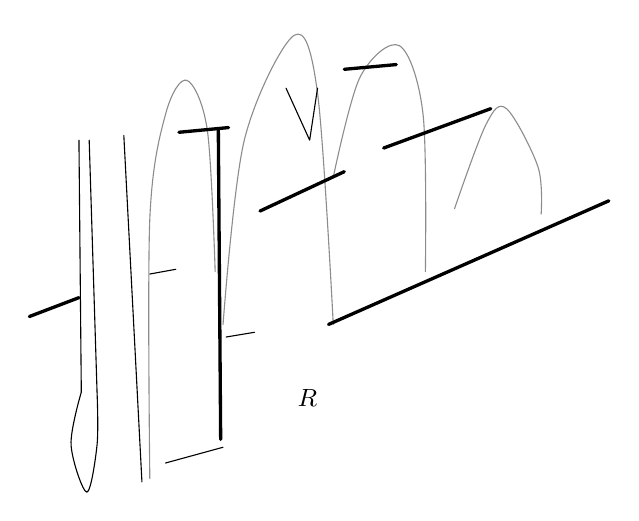
\begin{tikzpicture}[x=1mm,y=1mm,line cap=round,line join=round,font=\scriptsize]
\draw[pencil] plot[smooth, tension=0.55] coordinates {(40,-96.3) (40,-63.3) (42,-50) (44.7,-45.7) (47.3,-52) (48.3,-70)};
\draw[pencil] plot[smooth, tension=0.55] coordinates {(49.3,-76.7) (52,-53.3) (58.3,-40) (61.3,-47.3) (63.3,-76.7)};
\draw[pencil] plot[smooth, tension=0.55] coordinates {(63.3,-58) (66.7,-45.3) (71.7,-41.3) (74.7,-50) (75,-70)};
\draw[pencil] plot[smooth, tension=0.55] coordinates {(78.7,-62) (82.7,-51.3) (85.3,-49.3) (89.3,-56.7) (89.7,-62.7)};
\draw (31,-53.3) -- (31.3,-85.3);
\draw (32.3,-53.3) -- (33.3,-85.3);
\draw plot[smooth, tension=0.55] coordinates {(31.3,-85.3) (30,-92) (32,-98) (33.3,-92) (33.3,-85.3)};
\draw (36.7,-52.7) -- (39,-96.7);
\draw[very thick] (48.7,-52) -- (49,-91.3);
\draw[very thick] (24.7,-75.7) -- (31,-73.3);
\draw[very thick] (43.7,-52.3) -- (50,-51.7);
\draw (40,-70.3) -- (43.3,-69.7);
\draw (49.7,-78.3) -- (53.3,-77.7);
\draw (42,-94.3) -- (49.3,-92.3);
\draw[very thick] (54,-62.3) -- (64.7,-57.3);
\draw[very thick] (64.7,-44.3) -- (71.3,-43.7);
\draw (57.3,-46.7) -- (60.3,-53.3) -- (61.3,-46.7);
\draw[very thick] (69.7,-54.3) -- (83.3,-49.3);
\draw[very thick] (62.7,-76.7) -- (98.3,-61);
\node[inner sep=1pt] at (60,-86) {\small $R$};
\end{tikzpicture}
\end{document}
